\subsection{Updated Methodology}
\begin{frame}
    \frametitle{Introduce and update capacity factors}
    The current methodology matches installed capacity to a demand 
    in the energy generated. Need to introduce capacity factors to 
    match energy generated to a demand in energy generated.
    \begin{itemize}
        \item Assume \glspl{LWR} operate at a 92.66\% 
              \gls{CF} \cite{us_eia_monthly_2022}
        \item Assume Xe-100 and VOYGR operate at 95\% \gls{CF}
              \cite{xenergy_reactor_nodate,nuscale_technology_nodate}
        \item Assume the \gls{MMR} operates at 100\% \gls{CF}
        \item Do not explicitly model outages for any reactor, extend 
              operating cycle by 1 month for \glspl{LWR} and VOYGRs
        \item This methodology changes the energy supplied by \glspl{LWR}, 
              slightly changes the number of reactors deployed,
              but does not affect the amount of fuel or when the reactors 
              receive fuel. 
    \end{itemize}
\end{frame}

\begin{frame}
    \frametitle{Effect of updated methodology}
    \begin{columns}
        \column[t]{5cm}
            \begin{itemize}
                \item The energy demand changes to 87.20 GWe-yr (previously 
                      89.46 GWe-yr) because 
                      of the updated LWR \gls{CF}
                \item All of the scenarios meet the minimum demand or 
                      provide an oversupply of power
                \item There is little variation in the energy supplied
                      in each scenario
            \end{itemize}
        \column[t]{5cm}
        \vspace{-0.8cm}
            \begin{figure}
                \centering
                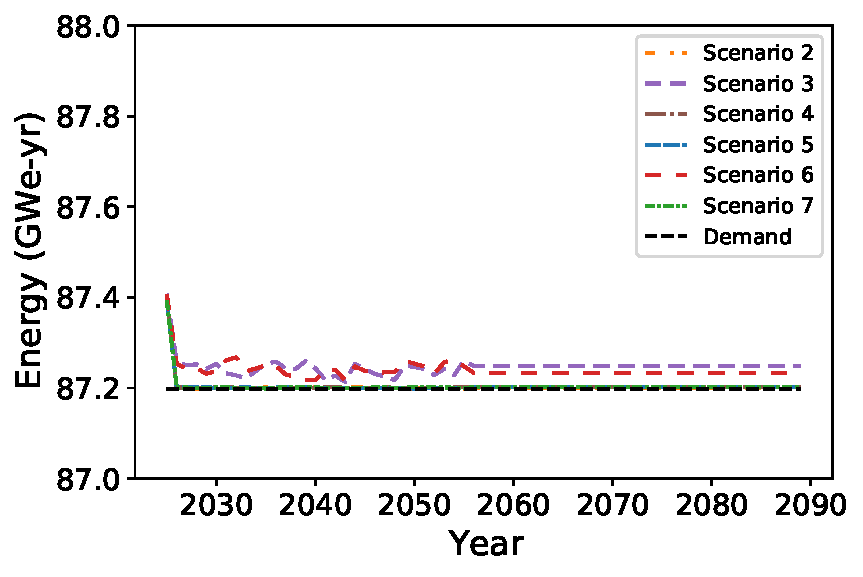
\includegraphics[scale=0.4]{updated_energy_after_2025.pdf}
                \caption{Annual average energy produced (GWe-yr) in Scenarios 
                2-7 compared with energy demand}
                \label{fig:updated_energy}

        \end{figure}
    \end{columns}
\end{frame}

\subsection{Summary}
\begin{frame}
\frametitle{Summary}
Preliminary work investigates the material requirements 
of transitioning from \glspl{LWR} to different 
subsets of advanced reactors.
\begin{itemize}
        \item Primarily deploying VOYGRs increases the amount of 
              fuel required but decreases the mass of \gls{HALEU}
        \item Deploying primarily Xe-100s or VOYGRs results in 
              similar feed uranium and \gls{SWU} requirements
        \item Deploying \glspl{MMR} greatly increases the number of 
              reactors, feed uranium, and \gls{SWU} capacity required
        \item For a 1\% growth in energy demand, similar trends are 
              observed
\end{itemize}
However, the preliminary work has some limitations:
\begin{itemize}
        \item Only considers once-through fuel cycle
        \item Only considers changes in the energy demand and
              reactors deployed
        \item Only considers enriching natural uranium to produce 
              \gls{HALEU}
\end{itemize}
\end{frame}